\chapter[The CMS experiment at LHC]{The CMS experiment at LHC}

The CMS experiment is one of the biggest particle physics experiments on the world. It is located at the ring of the LHC that is the main accelerator managed by CERN, the European Organization for Nuclear Research or Centre Europ\'{e}enne pour la Recherche Nucl\'{e}aire by its french name. This center constitutes the biggest center for research on particle physics all over the world. All along its 60 years of existence, from 1954, 21 member states have been joining it, but an overall of 113 countries participate in different ways on this center. 

On the present chapter we discuss in detail different aspects of the LHC accelerator and the CMS experiment. In particular we make some emphasis in the CMS sub-detectors related to jets, objects that play the main role on the search that is the main subject of the present work. We also discuss the present state of both machines, their achievements and the challenges that were overcome. Finally, also the expectations and goals for the upcoming run II are mentioned.  

\section{The Large Hadron Collider}
\label{sec:LHC}

The Large Hadron Collider, or LHC~\cite{Bruning:782076}, is a machine that accelerates and collides protons and lead. This machine is the biggest particle collider nowadays with a circumference of 27 km. It also achieves the highest energy by a collider up to present, planned to be 14 TeV at the center of mass of the collision. On the first run of the machine only 8 TeV were achieved, and next run is planned to start with 13 TeV. It's located in French-Swiss border near to Geneva. The tunnel for the machine was carved around 100 m under the ground, 45 m under the Jura mountains and 170 m under the L\'{e}man lake with an inclination of around 1.4\%, sloping down towards the lake . This machine has used as much as possible old LEP buildings and sites, that was an electron-positron collider built between 1984 and 1989. 

The protons and heavy ions accelerated by the machine collide in different points where dedicated experiments are located to detect and study the product from the collisions. The four main experiments located on the LHC ring are CMS~\cite{Bayatian:922757,Bayatian:942733}, ATLAS~\cite{ATLAS:1999}, LHCb~\cite{Alves:2008zz} and ALICE~\cite{Cortese:879894}. The first two are experiments of generic purpose where searches for new physics and also precision measurements are performed. LHCb is dedicated to the physics of the b-quark, and ALICE focuses on the study of the quark-gluon plasma produced from heavy ions collisions. Even if one of the principal objectives of the construction of the LHC was the search for the Higgs boson, generic searches on new physics have been conducted from the very beginning of the first data taking in 2009. Moreover, after the Higgs discovery in 2012 there is a growing effort on the searches for new physics and precision measurement of the properties of the Higgs.

The LHC is a complex machine composed of several parts. The two principal parts are the injector chain and the main ring. A diagram of the whole CERN complex can be seen in figure~\ref{fig:Complex}. The injector chain has different stages that pre-accelerate protons and heavy ions to be injected into the main ring of LHC. %In the main ring the protons and heavy ions are fully accelerated and collided in four different points over the ring.

\begin{figure}[!Hhtbp]
  \begin{center}
    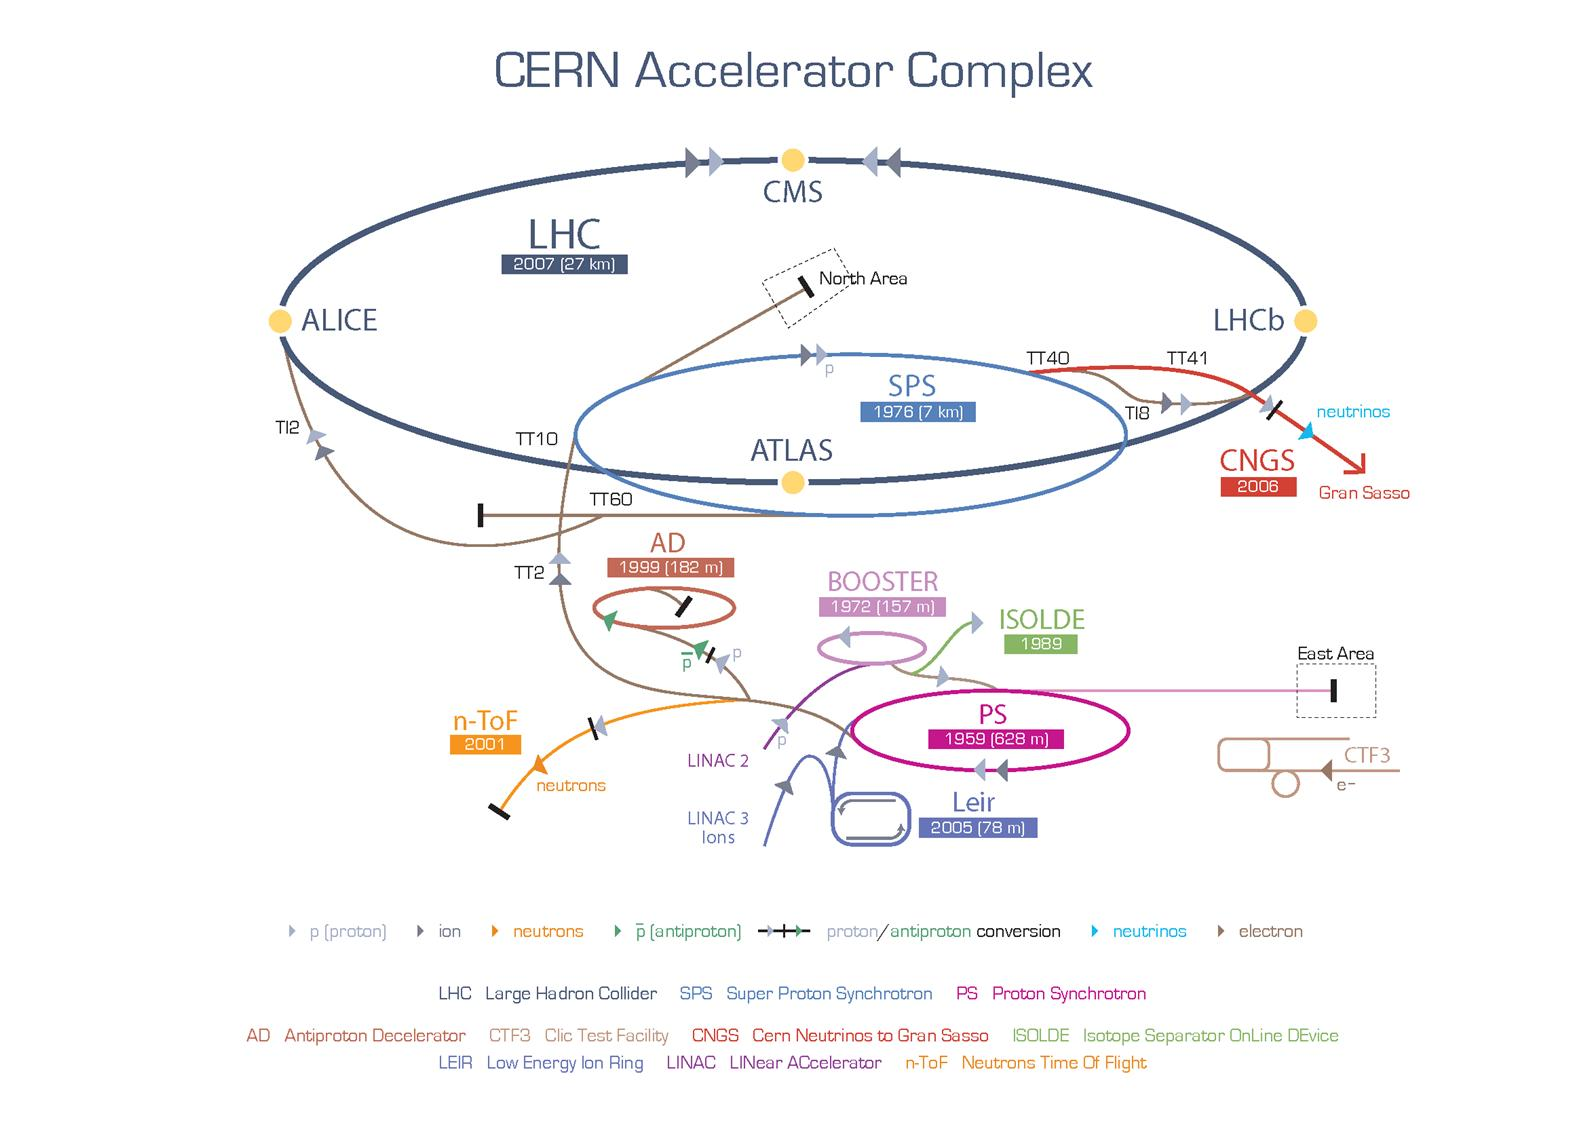
\includegraphics[trim=4.5cm 0cm 0cm 0cm, clip=true, width=1.15\textwidth]{figs/cern-lhc-4.jpg}
    \caption{Organization of CERN accelerator complex}
    \label{fig:Complex}
  \end{center}
\end{figure}

\subsection{Injector chain}
\label{sec:injector}

The injector chain begins with the proton source. Protons are extracted via ionization of Hydrogen gas in the Duoplasmatron Proton Ion Source. Such extraction is pulsed, what makes up the first bunch structure. The extracted protons are then accelerated up to 50 MeV in the linear accelerator, Linac2, that dates from 1978. After this first stage several steps are followed:
\begin{enumerate}
\item Linac2 injects proton bunches in the Proton Synchrotron Booster (PSB) where they are accelerated to 1.4 GeV. 
\item From PSB, the protons are delivered to the Proton Synchrotron (PS) where they reach an energy of 25 GeV. In the PS the bunches are also split from 6 initial bunches to 72 spaced by 25 ns.
\item Finally, the pre-acceleration chain is finished by the SPS, Super Proton Synchrotron. There the bunches are accelerated up to 450 GeV right before being inserted into the main LHC ring. 
\end{enumerate}

The whole pre-acceleration chain has been optimized to obtain the best possible performance on the final acceleration in the LHC main ring. All parameters are carefully controlled, for example the number of bunches, the separation between bunches, the separation between trains of bunches or the injection energy to each subsystem. It's also remarkable to notice the level of control achieved in the bunches manipulation, from old subsystems as the PS from 1959 or the newest, the SPS that dates from 1976. 

Some recent plans for future accelerator have been studied using the LHC main ring as injector for a bigger accelerator, for example the so called FCC (Future Circular Collider) at CERN. The FCC could be built perform proton-proton, electron-positron or electron-proton collisions, versions that are called respectively FCC-hh, FCC-ee and FCC-he. The FCC-hh is being designed to achieve 100 TeV of center of mass energy in a tunnel of 80-100 km of circumference. 

\subsection{Main ring}
\label{sec:ring}

The main ring is composed of two rings that accelerate the proton bunches in opposite directions, clock-wise and counter clock-wise. An schematic view of the design of the main ring can be seen in figure~\ref{fig:schematic}. The rings crosses in different points in order to collide the protons and they are divided in eight straight sections and eight arcs. In each octant bunches are controlled by dipole magnets. These complex magnets, in figure~\ref{fig:dipole}, need to produce a very strong magnetic field in order to be able to bend a 7 TeV beam of protons. This intense magnetic field, 8.33 T, in opposite directions, is produced by electrical currents that are only achievable by means of superconductivity. All the 1232 dipoles operate at a temperature of 1.9 K, under cooling by liquid helium. They also operate under ultra-high-vacuum. The beam lines with a pressure less than $10^{-9}$ mbar and the whole dipole system with $10^{-6}$ mbar, that serves also as insulating system from the surroundings. In addition, the LHC main ring has other magnets that focus and correct different characteristics of the beam: 520 quadrupoles, 2464 sextupoles, 1232 octupoles. 

\begin{figure}[!Hhtbp]
  \begin{center}
    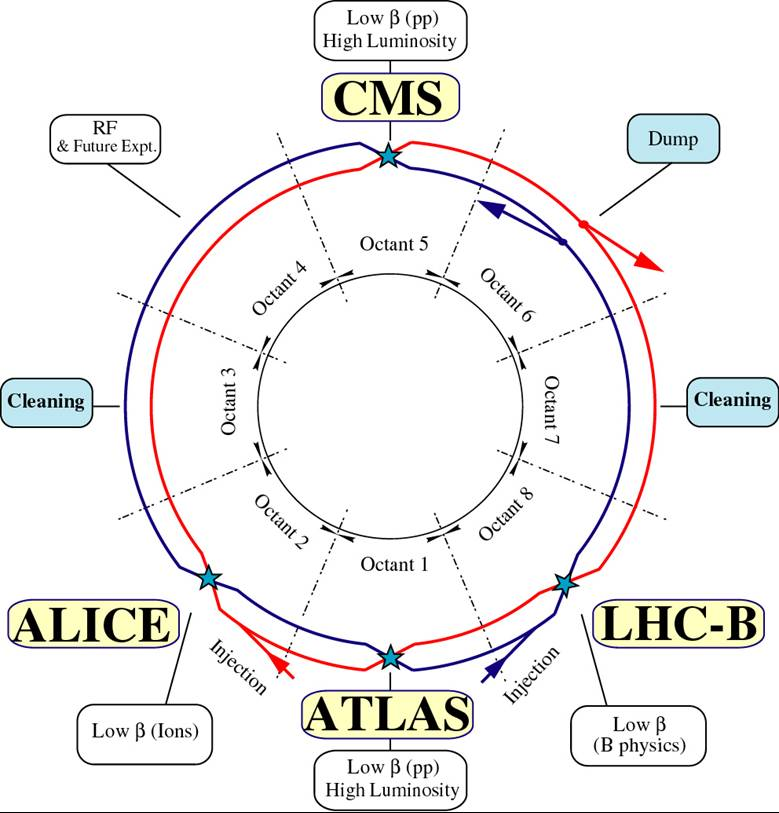
\includegraphics[width=0.8\textwidth]{figs/lhc-schematic.jpg}
    \caption{Schematic of the LHC main ring design.}
    \label{fig:schematic}
  \end{center}
\end{figure}

\begin{figure}[!Hhtbp]
  \begin{center}
    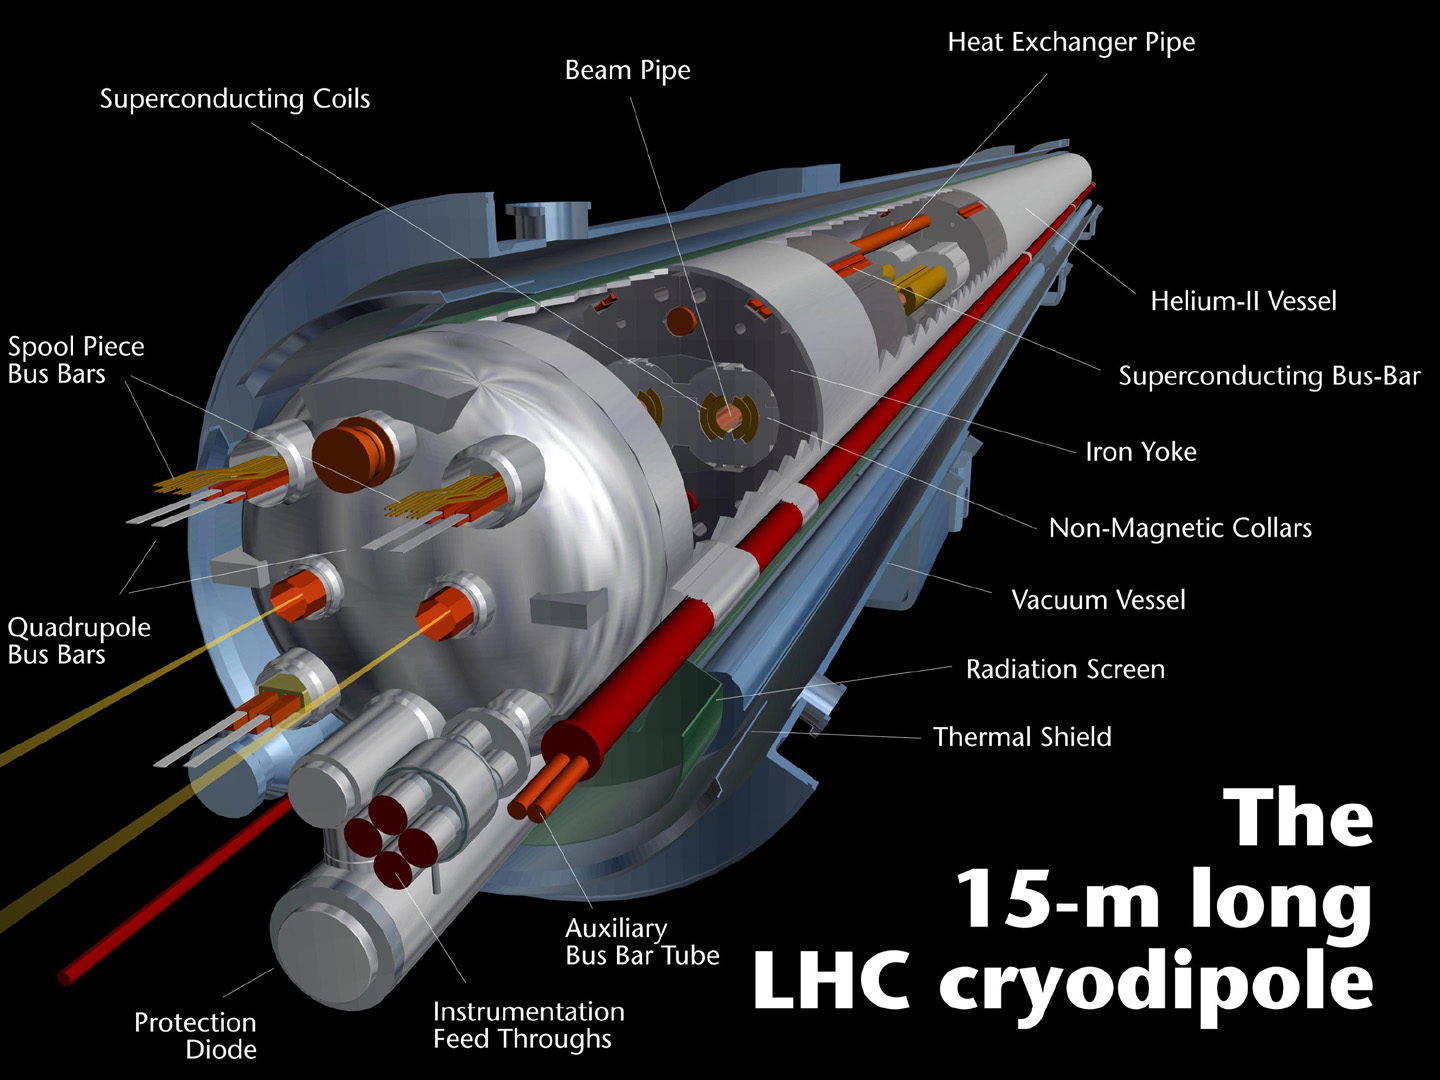
\includegraphics[width=0.45\textwidth]{figs/cryodipole.jpg}
    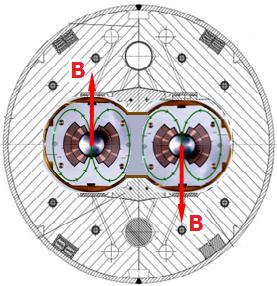
\includegraphics[width=0.45\textwidth]{figs/dipole_B.jpg}
    \caption{Design of LHC cryodipole and the magnetic field that bends the beam in the main ring.}
    \label{fig:dipole}
  \end{center}
\end{figure}

\subsubsection{Luminosity}
\label{sec:lumi}

In collider physics, such as the LHC, the figure of merit is the luminosity, given in equation~\ref{eq:lumiC}. The number of events per second is proportional to the luminosity, hence is the quantity to be maximized by the design and operation of the accelerator. The collider characteristics depend on the number of bunches in the ring $n_{b}$, the number of protons per bunch $N_{b}$, the revolution frequency $f_{rev}$, the relativistic gamma factor $\gamma$, the normalized rms transverse beam emittance $\epsilon_{n}$ and the beta function at the interaction point $\beta^{*}$. The denominator on~\ref{eq:lumiC} can also be rewritten in terms of the horizontal and vertical width of the bunches at the crossing, $\sigma^{*}_{x}$ and $\sigma^{*}_{y}$. In addition, there is the geometric reduction factor ($R$) that introduces a dependence on the crossing angle of the bunches at the interaction points. In table~\ref{tab:LHCparams} can be found the LHC beam parameters at injection and collision.  

\begin{equation}
  \label{eq:lumiC}
  L=\frac{n_{b}N_{b}^{2}f_{rev}\gamma}{4\pi\epsilon_{n}\beta^{*}}R=\frac{n_{b}N_{b}^{2}f_{rev}}{4\pi\sigma^{*}_{x}\sigma^{*}_{y}}R
\end{equation}

\begin{table}[htbH]
\label{tab:LHCparams}
\begin{center}
%\topcaption{LHC proton beam parameters.\label{tab:LHCparams}}
%\resizebox{\textwidth}{!}{
\begin{tabular}{|c|c c|}
\hline 
Parameter/units & Injection & Collision \\
\hline
Energy [GeV]& 450 & 7000 \\ 
Luminosity [$\text{cm}^{-2}\text{s}^{-1}$] & & $10^{34}$ \\
$k_{b}$ Number of bunches & \multicolumn{2}{c|}{2808} \\
Bunch spacing [ns] & \multicolumn{2}{c|}{24.95} \\
$N_{b}$ intensity per bunch [protons/bunch] & \multicolumn{2}{c|}{$1.15\times 10^{11}$} \\
Beam current [A] & \multicolumn{2}{c|}{0.58} \\
$\epsilon_{n}$ normalized rms transverse beam emittance [$\mu$m] & 3.5 & 3.75 \\ 
$f_{rev}$ revolution frequency [kHz] & \multicolumn{2}{c|}{11.25} \\
\hline
\end{tabular}
%}
\end{center}
\end{table}

At the crossing points, the number of events coming from collisions and produced via a specific process, is directly proportional to the luminosity provided by the collider, as in equation~\ref{eq:lumiC}.

\begin{equation}
  \label{eq:lumiN}
  N_{events}=L\sigma_{process}
\end{equation} where $\sigma_{process}$ is the cross section of the process. 

The total cross section of a proton-proton collision from the crossing of two bunches at 14 TeV is 100-110 mb~\cite{Augier:1993ta}, from three different scattering processes: elastic, diffractive and inelastic. In the elastic scattering the protons only exchange momenta but their structure remain unchanged, that is the case for the majority of collisions. In diffractive scattering momenta is exchanged and also new particles are produced in addition to the two final protons. Finally, in inelastic scattering, the constituents of the protons, the partons, interchange a big amount of momentum and produce a large quantity of particles. The inelastic processes contribute less than diffraction to the total cross section. While inelastic collisions produce particles in the central rapidity (defined in~\ref{sec:Csys}) region, diffractive and elastic final products have a large rapidity. Only in the hard interactions, inelastic scattering, color is exchanged, being the reason to fill up the central rapidity region. 

From the crossing of two bunches not only one proton-proton interaction is expected. In average, 25 interactions are expected for each crossing. From them, only one is coming from an inelastic collision, that is the type of process of more interest for detectors as CMS or ATLAS. This fact puts an additional difficulty to the detectors in order to extract the hard interaction from all the elastic and diffractive collisions happening at same time. Such phenomena is known as Pile-Up, an illustration of a collision with high pile-up can be found on figure~\ref{fig:pileup} as seen by the CMS detector.

\begin{figure}[!Hhtbp]
  \begin{center}
    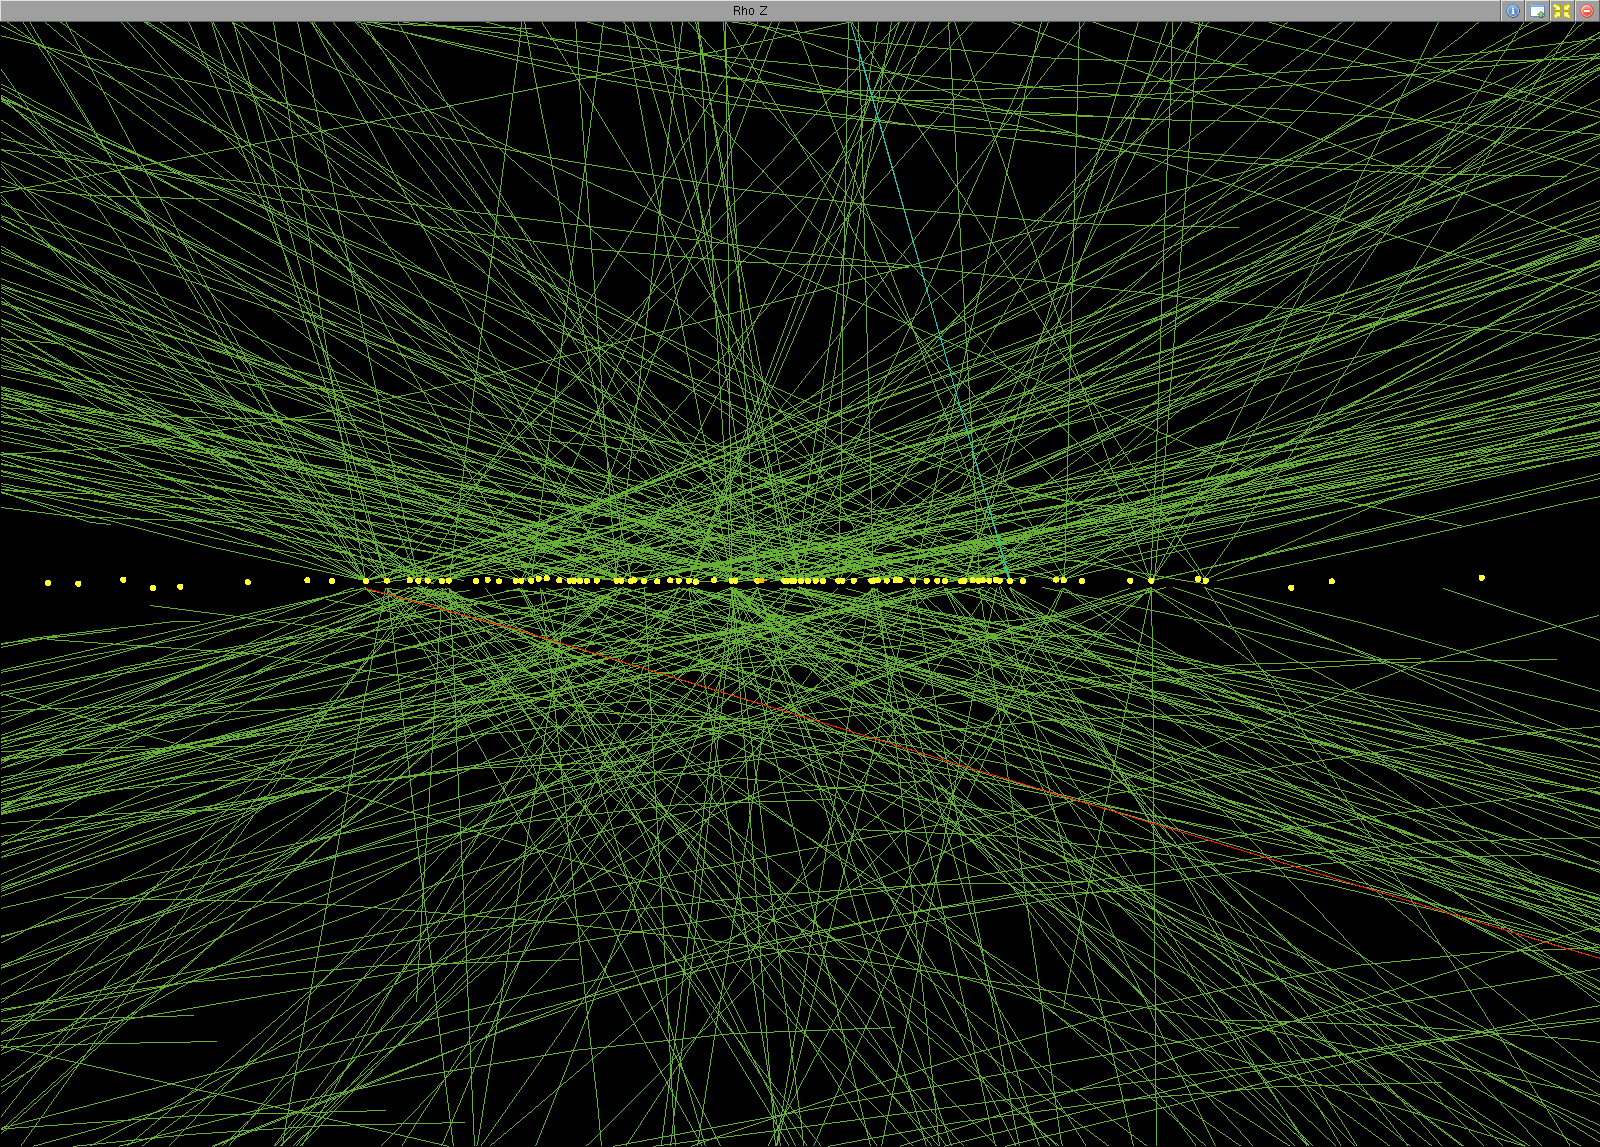
\includegraphics[width=0.7\textwidth]{figs/pileup.png}
    \caption{High pile-up event (78 interactions) seen by CMS detector. Event 35655522, from 198609 run, lumi 56, recorded on 2012. Image credit: Andre Holzner \copyright CERN}
    \label{fig:pileup}
  \end{center}
\end{figure}

\subsection{Run 1}
\label{sec:run1}

On February 10 of 2013 the first stable run of the LHC reached an end. This run, now called Run 1, started on November 20 of 2009. LHC was originally planned to start in 2008, but an incident on one of the electric connections of one of the magnets forced to stop on the 19th of September of the same year. From the restart in 2009, the energy was augmented from 450 GeV to 4 TeV per beam. The 23th of September 2009 the first collisions were detected by the experiments. One week after, the achieved center of mass energy was $\sqrt{s}=2.36$ TeV, already higher than Tevatron (0.98 TeV).

In 2010, from 30th March to 6th December 3.5 TeV per beam were reached delivering near 50 $\text{pb}^{-1}$. With the same energy, approximately 6 $\text{fb}^{-1}$ were delivered in 2011. 

In 2012, the center of mass energy reached one additional TeV, $\sqrt{s}=8$ TeV, and around 20 $\text{fb}^{-1}$ of integrated luminosity were delivered between April and December. On figure~\ref{fig:CMSlumi} can be seen the progress of the recorded luminosity by CMS for 2010-2012 period. The first six weeks of 2013 were devoted to proton-lead collisions.

After this very successful run, the LHC has been stopped for more than a year for repair and maintenance of different systems in the experiments and in the LHC itself to achieve higher energies. After this period, known as Long Shutdown  or LS1, the LHC is planned to restart a new run on the early spring of 2015.

\begin{figure}[!Hhtbp]
  \begin{center}
    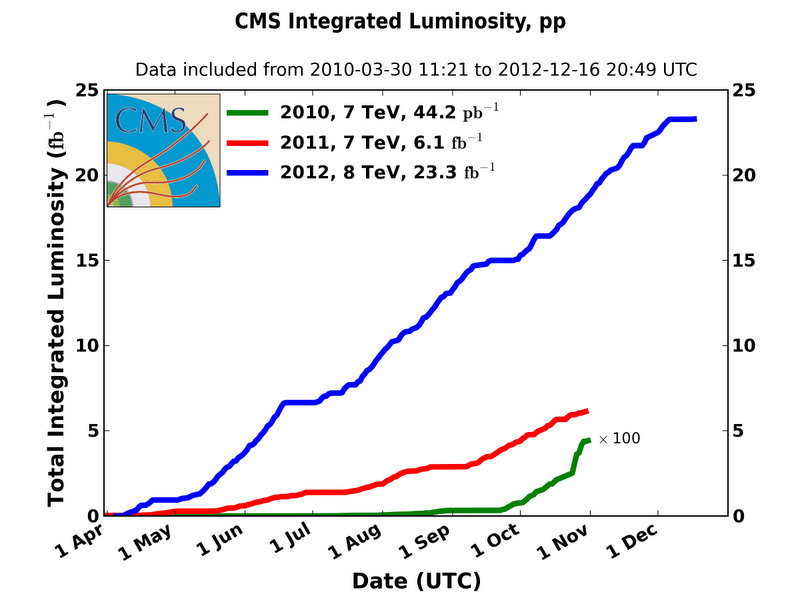
\includegraphics[width=0.7\textwidth]{figs/cms-int-10to12.jpg}
    \caption{CMS integrated luminosity for proton-proton collisions delivered by LHC. \copyright CERN}
    \label{fig:CMSlumi}
  \end{center}
\end{figure}

\subsection{Other experiments at LHC}
\label{sec:expers}

On the main ring there are several experiments depending on the collisions delivered by the LHC main ring. The biggest are CMS~\cite{Bayatian:922757} and ATLAS~\cite{ATLAS:1999}, both of them generalist experiments designed to do precision measurements as well as new physics searches. Mainly recording proton-proton collisions, they have also recorded lead-lead and proton-lead collisions during the run 1. Both of them were designed for high instantaneous luminosity, $L = 10^{34}\text{cm}^{2}\text{s}^{-1}$.

In addition, there is two other experiments designed for specific purposes. The LHCb~\cite{Alves:2008zz} that focus on the study of the physics of the b-hadrons, specially related to the CP violation, and ALICE~\cite{Cortese:879894} built for the study of strongly interacting matter. The first of them record proton-proton collisions at an instantaneous luminosity of $10^{32}\text{cm}^{2}\text{s}^{-1}$ and the second record ion-ion collision with $L = 10^{27}\text{cm}^{2}\text{s}^{-1}$.

The CMS experiment is going to be described in detail in section~\ref{sec:CMS}. In the following sections we are going to present very briefly the other three experiments mentioned above. 

\subsubsection{ATLAS}
\label{sec:atlas}

The ATLAS experiment (A Toroidal LHC ApparatuS) is the biggest LHC experiment. It's located at point one, as displayed on figure~\ref{fig:schematic}, on the LHC main ring. It's a cylindrical detector similar to CMS, about 45 meter long, 25 meter high, and weights around 7000 tons. ATLAS main components are, from inside to outside, a tracking system, an electromagnetic calorimeter, a hadron calorimeter and muon chambers. In between this subsystems there is an internal solenoidal magnet and a set of external toroidal magnets. The detector design is presented on figure~\ref{fig:atlasdet}.

\begin{figure}[!Hhtbp]
  \begin{center}
    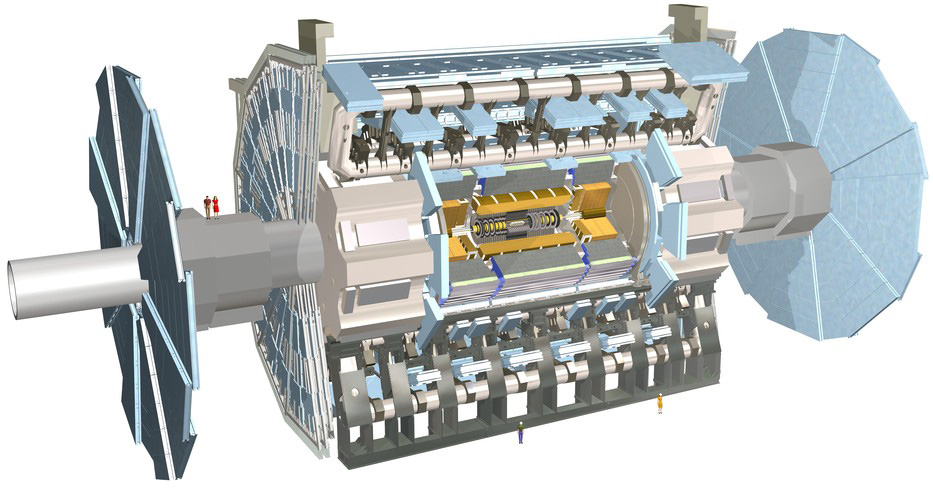
\includegraphics[width=0.7\textwidth]{figs/atlas_lg.jpg}
    \caption{ATLAS detector internal view. \copyright CERN}
    \label{fig:atlasdet}
  \end{center}
\end{figure}

On the human resources side, ATLAS experiment configures a collaboration of around 3000 persons, coming from 117 universities around the world, from 38 countries. Thirty percent of the collaboration are students.  

\subsubsection{LHCb}
\label{sec:lhcb}

LHCb detector, hosted at point 8 of the LHC main ring, has a different design than CMS and ATLAS. Smaller than these, its design mainly focus to be able to detect particles produced close to the beam direction. This is the reason why it is not cylindrically but conically shaped, in two detection arms~\ref{fig:lhcbupview}. It also has the same main parts, a tracking system with a very precise vertex locator, electromagnetic and hadron calorimeters, muon chambers and magnets. Its major specificity is a system that allows to identify different hadrons, what is crucial for the study of strong interacting matter. It measures 21 m long, 10 m high and 13 m wide, and weights 4500 tons. A view of the detector can be found on figure~\ref{fig:lhcbdet}. The LHCb collaboration groups around 700 persons from 50 different universities over 15 countries. 

\begin{figure}[!Hhtbp]
  \begin{center}
    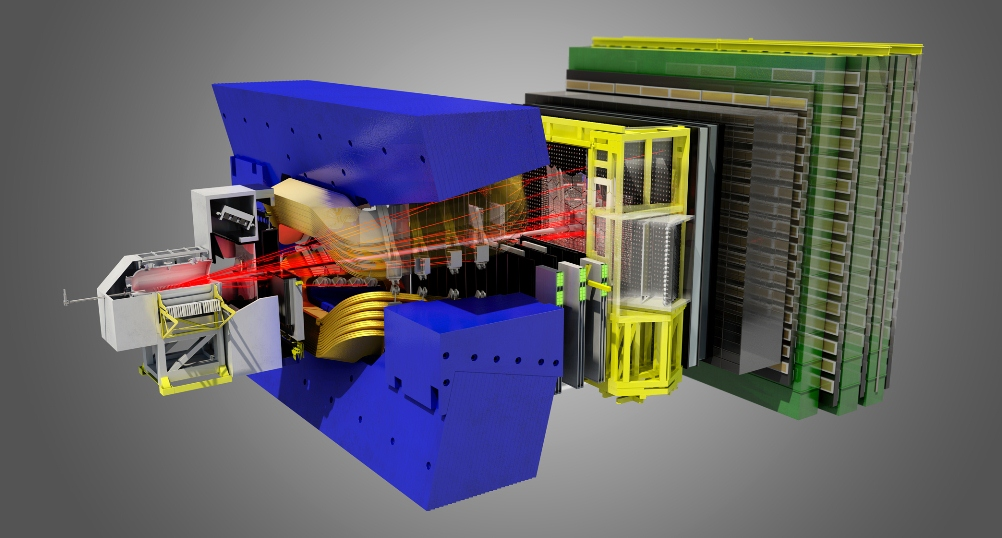
\includegraphics[width=0.7\textwidth]{figs/LHCbDetectorlight1.jpg}
    \caption{LHCb detector internal view. \copyright CERN}
    \label{fig:lhcbdet}
  \end{center}
\end{figure}

\begin{figure}[!Hhtbp]
  \begin{center}
    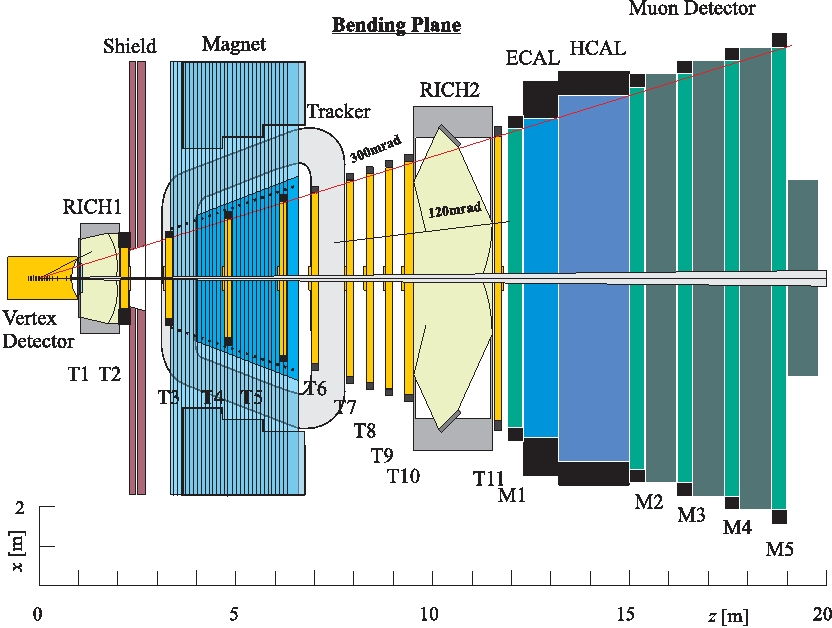
\includegraphics[width=0.7\textwidth]{figs/LHCb_UpView.jpg}
    \caption{LHCb detector view from the top. \copyright CERN}
    \label{fig:lhcbupview}
  \end{center}
\end{figure}

\subsubsection{ALICE}
\label{sec:alice}

The ALICE experiment (A Large Ion Collider Experiment) is located at point 2 of the LHC main ring, measures 16 m high, 16 m wide and 26 m long, and weights 10000 tons. It's an asymmetrical detector as LHCb. Its structure can be seen on figure~\ref{fig:alicedet}. ALICE collaboration counts around 1500 people, from 154 physics institutes in 37 countries. 

\begin{figure}[!Hhtbp]
  \begin{center}
    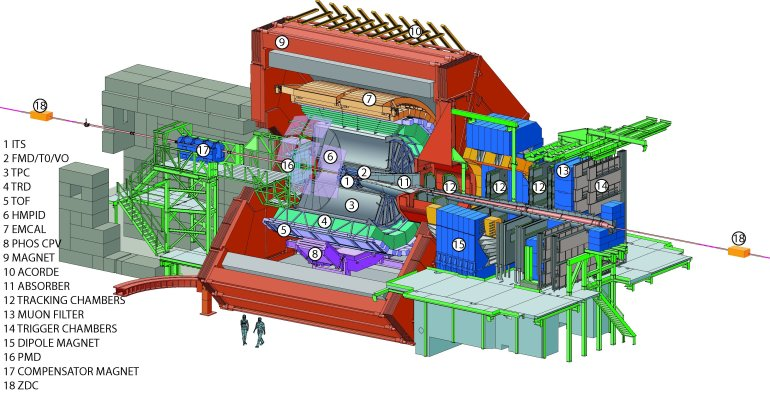
\includegraphics[width=0.7\textwidth]{figs/alice2.jpg}
    \caption{ALICE detector internal view. \copyright CERN}
    \label{fig:alicedet}
  \end{center}
\end{figure}

\section{The Compact Muon Solenoid (CMS) experiment}
\label{sec:CMS}

The CMS detector, hosted at point 5 of the LHC main ring (see figure~\ref{fig:schematic}), is the second biggest LHC experiment. Cylindrically shaped, measures 15 m of diameter and 28.7 m long, and weights 14000, making it the heaviest LHC experiment. Its subsystems are concentrically located from the collision point in the beam line. Its main characteristic is the strong 3.8 T solenoid magnet. A representation of the detector can be found in figure~\ref{fig:cmsdet}. The CMS collaboration is formed by around 2600 scientists, of which 900 are students, from 181 institutes over 41 countries. 

\begin{figure}[!Hhtbp]
  \begin{center}
    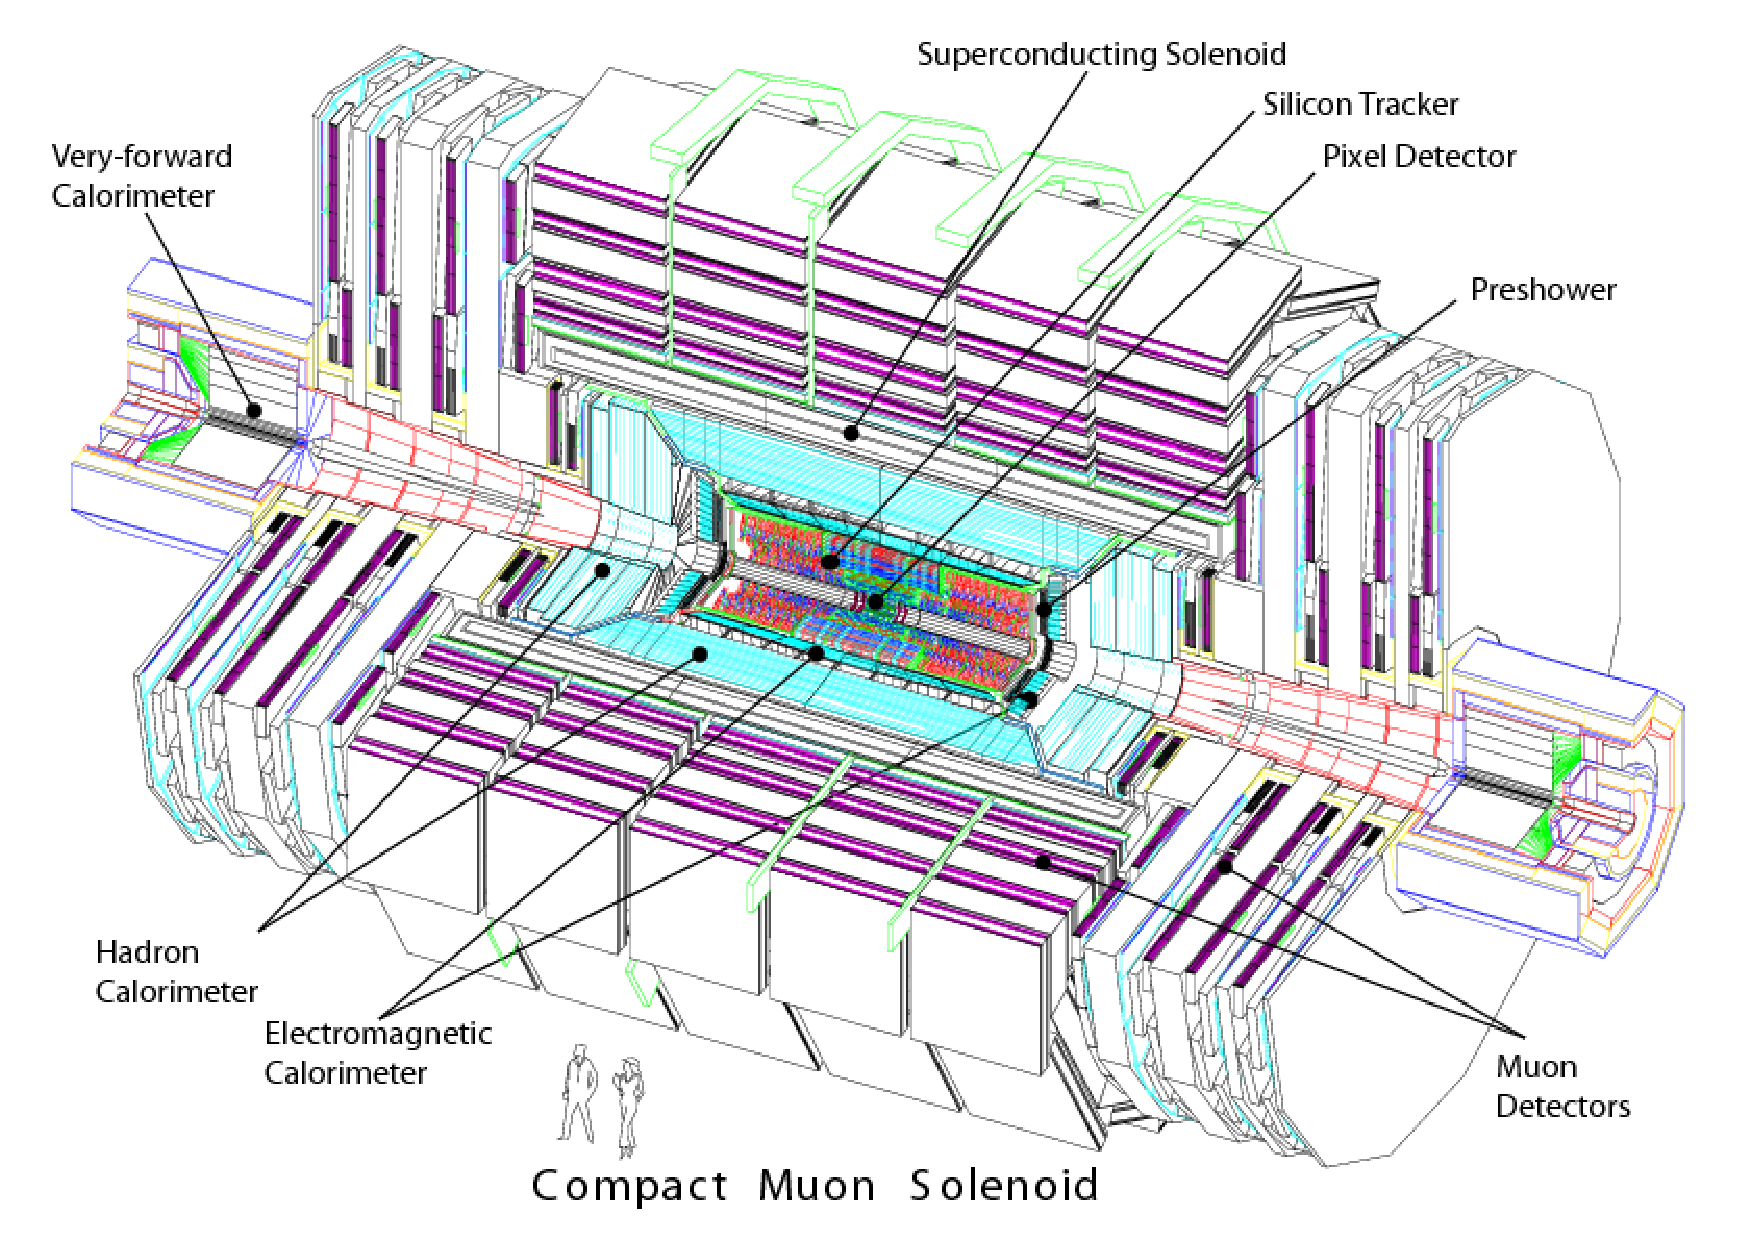
\includegraphics[width=\textwidth]{figs/CMS_det.pdf}
    \caption{CMS detector internal view. \copyright CERN}
    \label{fig:cmsdet}
  \end{center}
\end{figure}

CMS has been designed to be able to do very precise identification of particles originated from the collisions and their properties. For the measurement of the momentum of the charged particles, CMS counts with a very strong magnet that allows to bend very energetic particles. In addition, the calorimeters allow to measure accurately the energy from hadrons, electrons and photons. At the most external layer, the muons chambers measuring muons properties, and in the innermost the tracking system that reconstructs the collision points and the charged particles tracks. In figure~\ref{fig:cmsslice} can be found a representation of the different subsystems of CMS and how particles are reconstructed from them.

\begin{figure}[!Hhtbp]
  \begin{center}
    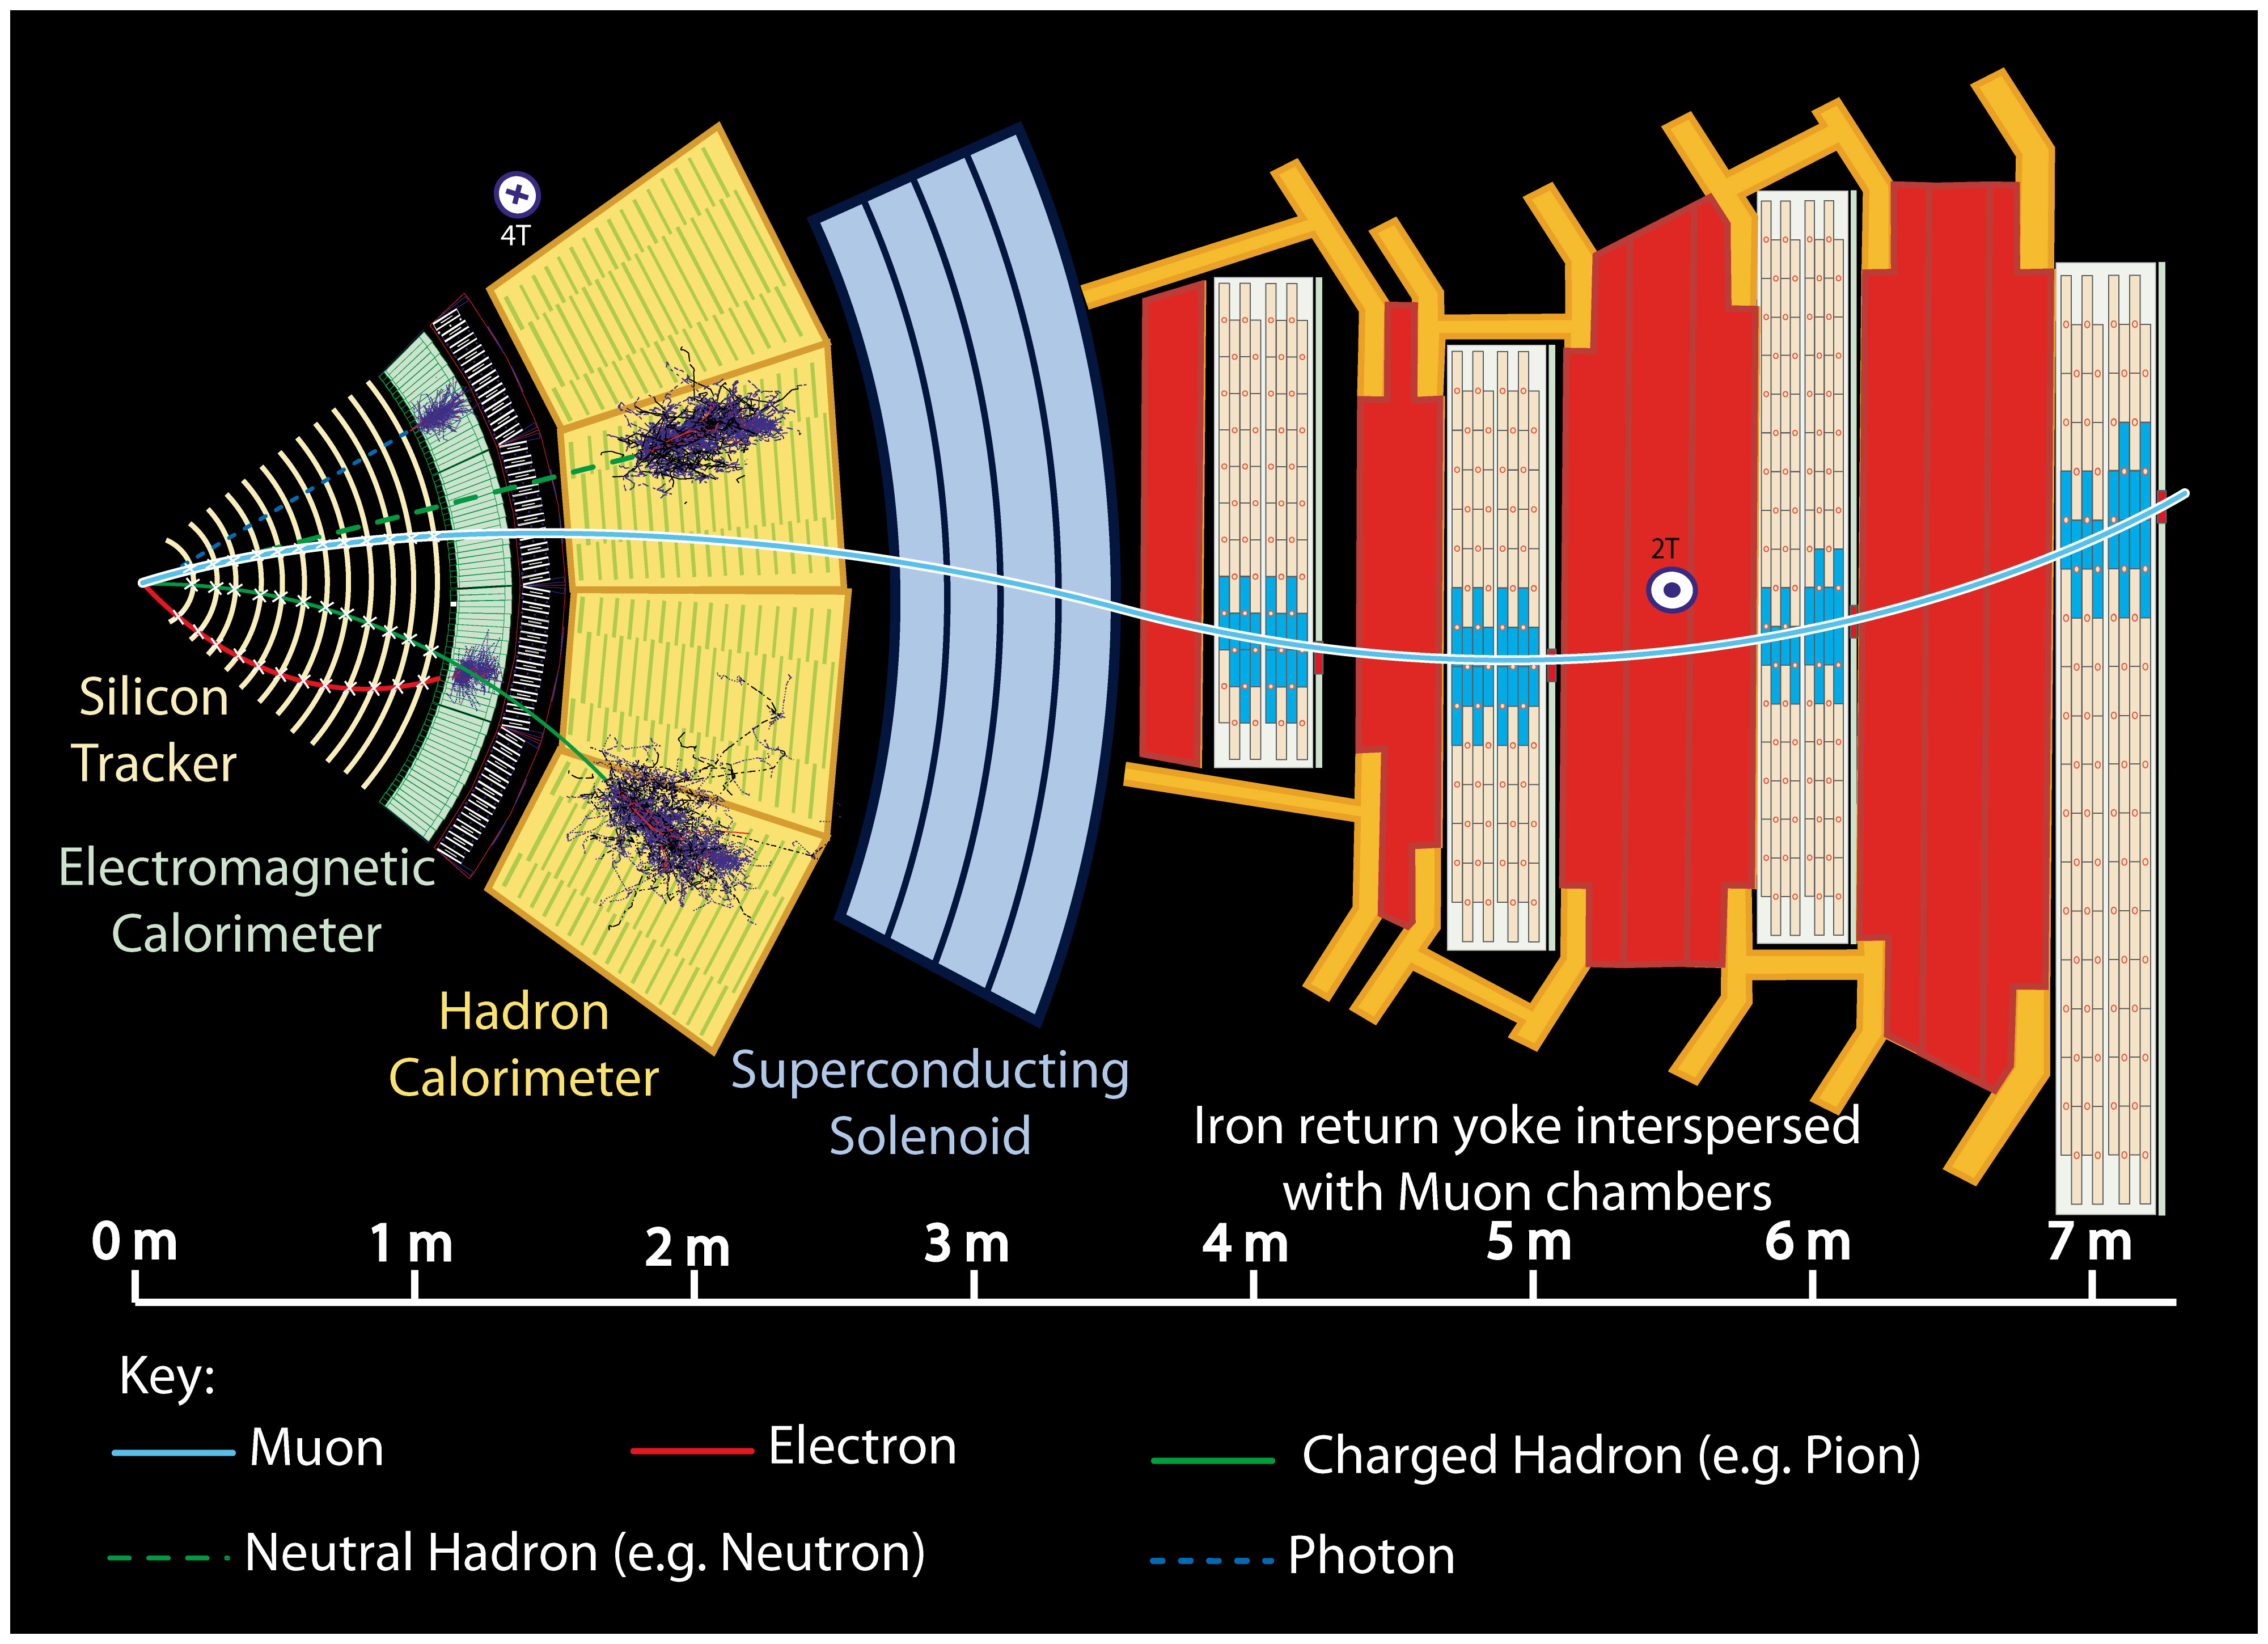
\includegraphics[width=\textwidth]{figs/PictureforPoint5_oct04_allp.jpg}
    \caption{CMS sub-detectors and particle identification. \copyright CERN}
    \label{fig:cmsslice}
  \end{center}
\end{figure}

\subsection{Coordinate system}
\label{sec:Csys}

The origin of coordinates defined on the CMS detector is located on the nominal collision point, the ``interaction point''. From there, the z-axis is defined along the beam pipe line pointing towards the Jura mountains. The positive/negative z-axis directions define the positive/negative sides of the detector. The y-axis is defined towards the zenith and the x-axis towards the center of the LHC ring. Due to the inclination of the LHC plane, this coordinate system is slightly tilted with respect to the true vertical. A representation of the coordinate system definition can be found in figure~\ref{fig:cmscoor}. 

\begin{figure}[!Hhtbp]
  \begin{center}
    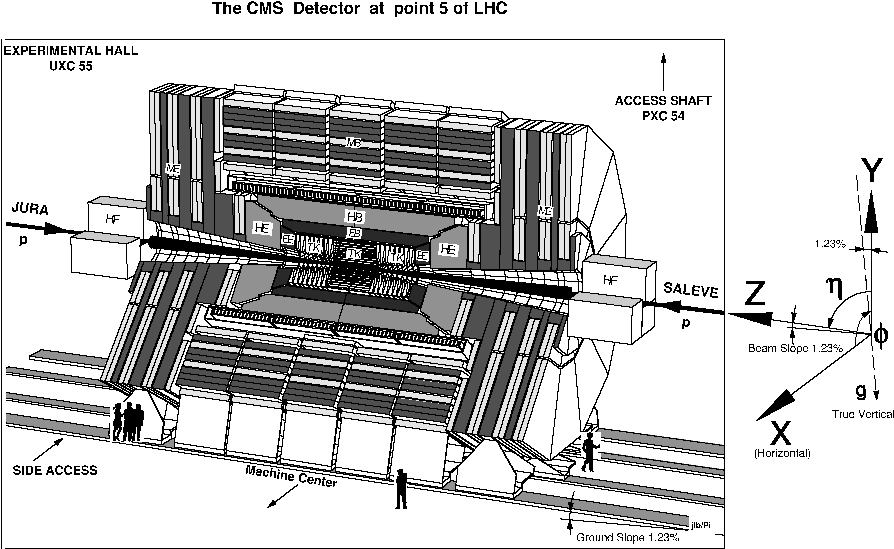
\includegraphics[width=\textwidth]{figs/CMS_coordinates.jpg}
    \caption{CMS coordinate system. \copyright CERN}
    \label{fig:cmscoor}
  \end{center}
\end{figure}

We can also define two angles: the $\phi$ angle in the x-y plane from the x-axis towards the positive y-axis, and the $\theta$ angle in the z-y plane from z-axis towards the positive y-axis. In experimental particle physics is preferred to work with relativistic invariant quantities, reason why instead of working with $\theta$ we define the pseudorapidity $\eta$, equation~\ref{eq:pseudorapidity}. 

\begin{equation}
  \label{eq:pseudorapidity}
  \eta = -\text{ln}\left( \text{tan}\left(\frac{\theta}{2}\right)\right)
\end{equation} 

One can define another relativistic invariant quantity, the rapidity $y$ as from equation~\ref{eq:rapidity}. With $\bm{p}$ being the momentum vector and $E$ the energy of a given particle, $p_{L}$ denotes its longitudinal component, that in our case is the same z-component. 

\begin{equation}
  \label{eq:rapidity}
  y=\frac{1}{2}\text{ln}\left(\frac{E+p_{L}}{E-p_{L}}\right)
\end{equation}On the limit that the mass of the particle is very small compared to its momentum, one can replace approximate the particle energy by the momentum magnitude, giving rise to the definition of the pseudorapidity in terms of the momentum of the particle $\eta = \frac{1}{2}\text{ln}\left(\frac{\bm{p}+p_{L}}{\bm{p}-p_{L}}\right)$

We define also the radial coordinate over the x-y plane, plane that is called the transverse plane being orthogonal to the longitudinal direction, the z-axis. In such plane are also defined the transverse quantities of particles, as the transverse momentum $p_{T}$. Finally, for any two objects an angular distance can be defined in the $\eta-\phi$ plane, as in equation~\ref{eq:deltaR}.

\begin{equation}
  \label{eq:deltaR}
  \Delta R=\sqrt{(\Delta\eta)^{2}+(\Delta\phi)^{2}}
\end{equation}

\subsection{Magnet}
\label{sec:magnet}

In order to measure the momentum of the charged particles going inside the detector is crucial to apply the correct magnet field, sufficiently strong to bend very energetic particles. The momentum of a charged particle inside an uniform magnetic field can be written as

\begin{equation}
  \label{eq:momB}
  p=\gamma m v=qBr
\end{equation} where $B$ is the magnitude of the magnetic field, $\gamma$ the usual relativistic factor, $m$ the mass of the particle, $v$ its rapidity, $q$ its charge and $r$ the bending radius. The sagitta of the arc is

\begin{equation}
  \label{eq:sagitta}
  s=\frac{L^{2}}{8r}=\frac{qBL^{2}}{8p}
\end{equation} with $L$ the distance the particle moved inside the magnetic filed. Inside a solenoid $L$ is equal to the radius of it. 

From relation~\ref{eq:sagitta} is possible to deduce that the resolution on the momentum of the particle has an inverse dependence with the magnetic field and the radius of the solenoid, as shown in equation~\ref{eq:presolution}. From there, for a better resolution is needed to increase the magnetic field and the radius of the solenoid. 

\begin{equation}
  \label{eq:presolution}
  \frac{dp}{p}\propto \frac{p}{BL^{2}}
\end{equation}

The design of CMS magnet target both features, it utilizes a large solenoid of 6 m of diameter and 13 m long. It's made of 4 layers of windings of NbTi cable that is cooled to 4.45 K in order to achieve the superconducting state. This magnet is able to produce an uniform magnetic field inside of it of 3.8 T. Outside the magnet 5 wheels and 3 disks of iron are placed in order to return the flux of the magnetic field, inducing just a 2 T radial magnetic field outside the solenoid. This iron yoke contributes with most of the weight of the detector, 10000 tons. In between the iron yoke the muon chambers are placed.  

\subsection{Tracker system}
\label{sec:tracker}

The tracker system has been designed to specifically address the reconstruction of high pt leptons, with particular interest in the isolation of electrons and, as a consequence, to isolate photons. Also the tracker fulfill granularity requirements to reconstruct secondary vertexes to tag and reconstruct B-hadrons. The tracker system is able to reconstruct tracks of particles with at least 2 GeV of $p_{T}$ with $|\eta|<2.5$. Charged hadrons are reconstructed with an efficiency of at least 85\% for $p_{T}=1$ GeV and up to 95\% for $p_{T}$ above 10 GeV. Another important point that was taken into account is the fact that the tracker is the part of CMS most exposed to radiation as it is the closest subsystem to the interaction point. The tracker system was built highly resistant to radiation damage and is expected to last for around 10 years. The pixel detector only lasts 2 years and was replaces during LS1. 

The tracker has been built with three different technologies: Pixels, Silicon Strips and Micro Strip Gas Chambers (MSGCs). They are arranged concentrically in cylindrical volumes being the pixel detector the innermost and the MSGCs the outermost. The CMS tracker extends to a radius of 155 cm and a around 270 cm on each $z$ direction. The pixel system is in the region with a radius below $\approx$ 20 cm, the silicon detector between $\approx 20$ cm and $\approx 60$ cm, and the MSGCs between $\approx 70$ cm and $\approx 120$ cm. The three subsystems are fast enough to work at 25 ns scale.

The pixel system is formed by three barrel layers and two end caps disks covering radii from 6 cm to 15 cm. It has an approximate active surface of one square meter with approximately $40\times10^{6}$ channels with a cell size of 150 $\mu$m by 150 $\mu$m. This pixel system allows to obtain three highly precise points that are mainly used for reconstructing vertexes.

The Silicon Strip system is formed by a 5-layer barrel (TIB for Tracker Inner Barrel) and 10 disks (TID for Tracker Inner Disks) in each end cap. The strips length is 12.5 cm with a pitch from 61 $\mu$m to 122 $\mu$m for single-sided strips and for 81 $\mu$m to 244 $\mu$m for double-sided. It's able to achieve a hit resolution of about 15 $\mu$m. 

The MSGCs systems is composed of 6 layers in the barrel (TOB for Tracker Outer Barrel) and 11 disks in each end cap (TEC for Tracker EndCap, with a $\pm$ sign depending on the $z$ direction). Here the strips are 10 cm length for the inner layers and 25 cm for outer layers with a pitch from 200 $\mu$m to 400 $\mu$m, which gives a hit resolution of 35 $\mu$m and 100 $\mu$m respectively. The MSGCs and Silicon systems have an overall active area of around 300 $\text{m}^{2}$ with 12 $\times10^{6}$ channels organized in more than ten thousand independent modules.

In figure~\ref{fig:cmstracker} can be seen the disposition of all the tracker subsystems. From the design of the tracker system the best resolution on the $p_{T}$ measurement is achieved in the $|\eta|<1.6$ region, this due to the presence of more layers of detector in the different subsystems, as shown in figure~\ref{fig:trackerres}. 

\begin{figure}[!Hhtbp]
  \begin{center}
    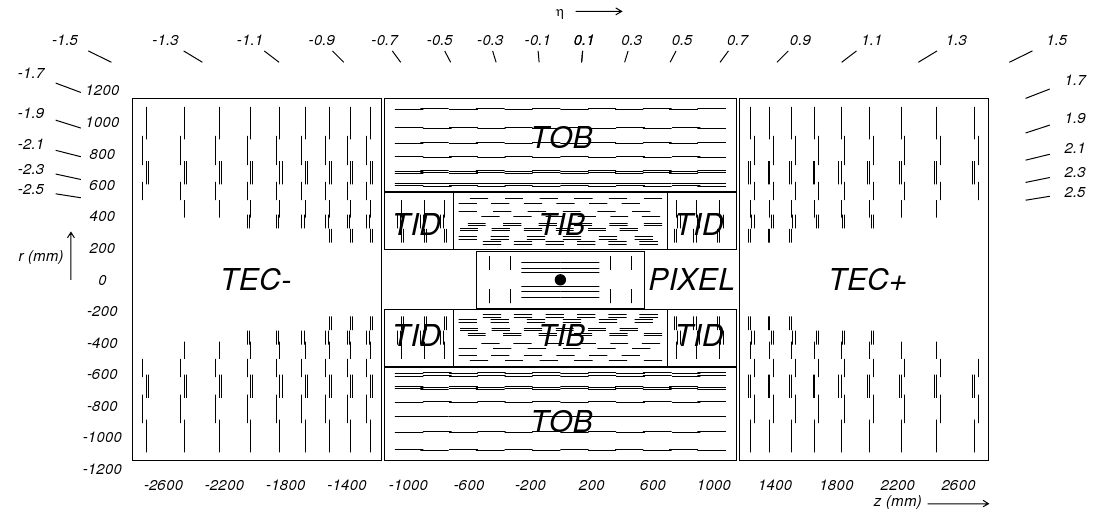
\includegraphics[width=0.9\textwidth]{figs/fig_cmstracker.png}
    \caption{CMS tracker system configuration. \copyright CERN}
    \label{fig:cmstracker}
  \end{center}
\end{figure}

\begin{figure}[!Hhtbp]
  \begin{center}
    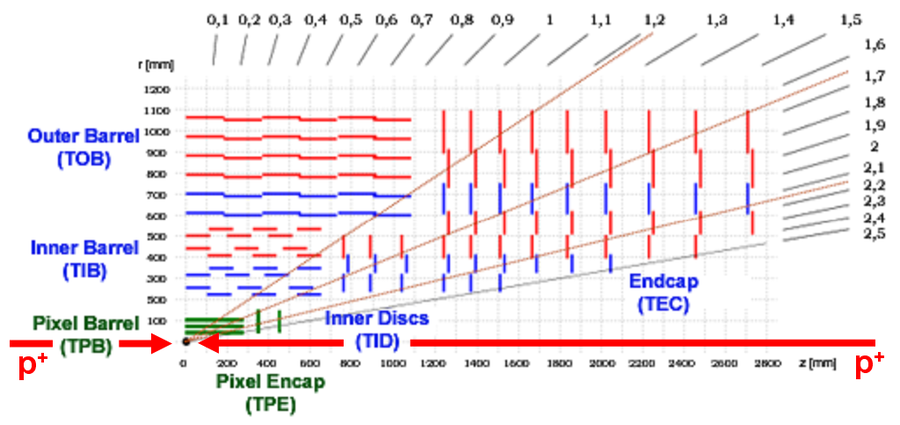
\includegraphics[width=0.9\textwidth]{figs/tracker_resolution.png}
    \caption{Tracker resolution with $\eta$. \copyright CERN}
    \label{fig:trackerres}
  \end{center}
\end{figure}

\subsection{Electromagnetic calorimeter}
\label{sec:ecal}

The CMS ECAL (Electromagnetic CALorimeter) is the detector subsystem designed to stop photons and electrons to measure their energy. It's an hermetic cylindrical calorimeter made of 61200 crystals in the barrel ($|\eta|<1.479$) and 7324 in each end cap ($1.48<|\eta|<3$). The crystals material is lead-tungstate that is transparent, very dense (8.28 g/$\text{cm}^{3}$), has a small Moliere radius (2.2 cm) and a short radiation depth ($X_{0}=0.89$ cm). This material has been chosen for the characteristics already described, but also because is very fast emitting the scintillation light (in 25 ns), it has a very good energy resolution and resistance to radiation. The crystals are distributed in 36 super-modules, 1700 crystals each, in the barrel (EB for ECAL Barrel) and in four 'Dee's, of 3662 crystals each, in the end caps (EE for ECAL End cap). In the EB the scintillation light is collected by Avalanche Photo-Diodes, or APD, and by Vacuum Photo-Triodes, or VPT, in the EE. A preshower system is installed in face of each end cap to allow a better discrimination between photons and $\pi^{0}$'s. A representation of the CMS ECAL can be found on figure~\ref{fig:ecal}.

\begin{figure}[!Hhtbp]
  \begin{center}
    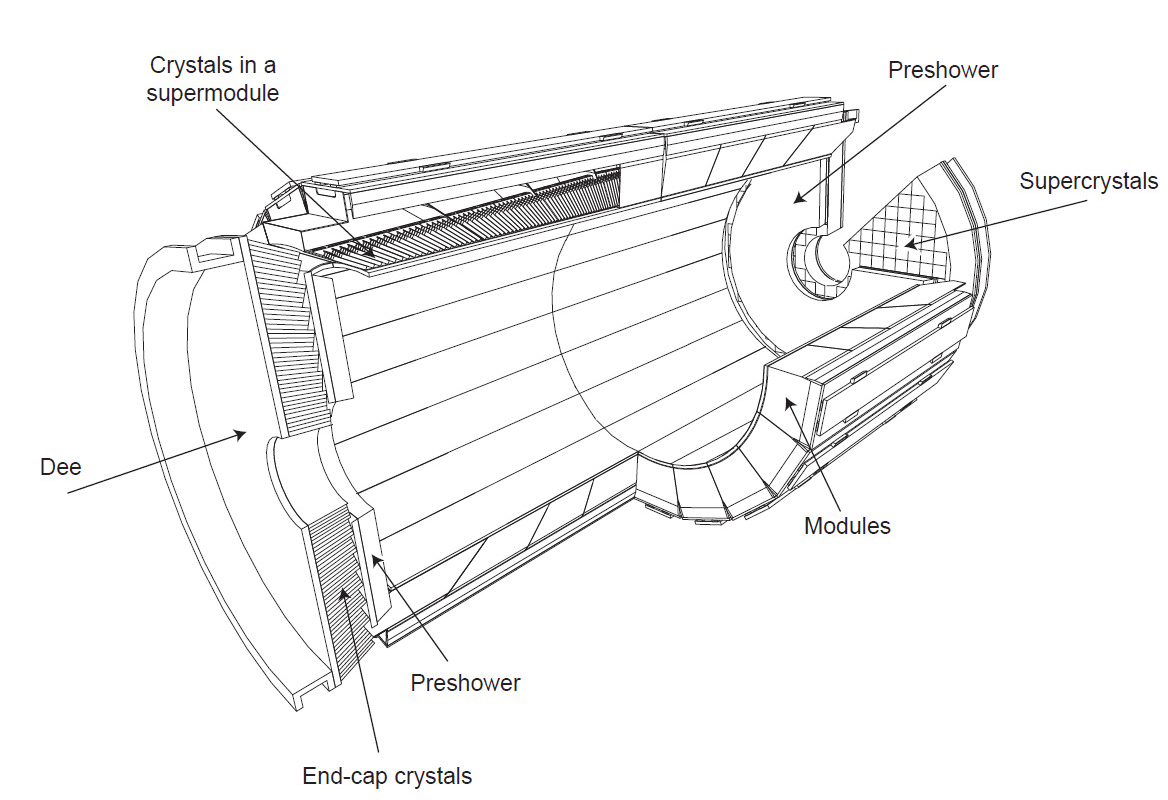
\includegraphics[width=0.9\textwidth]{figs/ECAL.png}
    \caption{CMS ECAL representation. \copyright CERN}
    \label{fig:ecal}
  \end{center}
\end{figure}

\subsection{Hadronic Calorimeter}
\label{sec:hcal}

The CMS HCAL, for Hadronic CALorimeter, is the subdetector designed to measure the energy of hadrons produced in the collisions, mainly the neutral hadrons because the charged hadrons are already traced by the tracker. It's also designed to measure the missing energy coming from particles not being detected by any of the subsystems, as neutrinos. It's an hermetic set of subsystems covering up to $|\eta|<5.2$:
\begin{itemize}
\item Hadron Barrel Calorimeter (HB): Covering $|\eta|<1.4$ is located between the ECAL barrel and the magnet. 
\item Hadron Endcap Calorimeter (HE): Extends the coverage of the barrel on the region $1.4<|\eta|<3$.
\item Hadron Outer Calorimeter (HO): Located outside the magnet, uses it as an additional absorber.
\item Hadron Forward Calorimeter (HF): Completes the coverage of the system from $|\eta|=3$ up to $|\eta|=5.2$.
\end{itemize}

The CMS HCAL layout is shown in figure~\ref{fig:hcal}. The system is made of two parts, an absorber to develop the hadronic showers and a scintillator to measure the particles energy. The length scale of hadronic calorimetry is designated as the interaction length corresponding to the mean free path of an hadron in a material. The HB absorber is made of 40 mm thick steel plate, eight layers of brass plates of 50.5 mm thick, six brass plates of 56.5 mm thick and a steel plate of 75 mm thick. The HE uses the same absorber but with thicker plates, of 79 mm. Between the absorber plates a plastic scintillator, Kuraray SCSN81, of 3.7 mm thick is placed. In the region with $|\eta|<1.6$ the achieved granularity is $\Delta\eta\times\Delta\phi=0.087\times 0.087$ and $\Delta\eta\times\Delta\phi=0.17\times 0.17$ in the region with $|\eta|>1.6$. This design gives a total of 70000 tiles used. The produced light in the HB is collected by optical fibers and transferred to the Hybrid Photo Diodes (HPDs). This diodes were chosen thanks to their small sensitivity to the magnetic field, an important feature due to the proximity of the HCAL to the magnet.

\begin{figure}[!Hhtbp]
  \begin{center}
    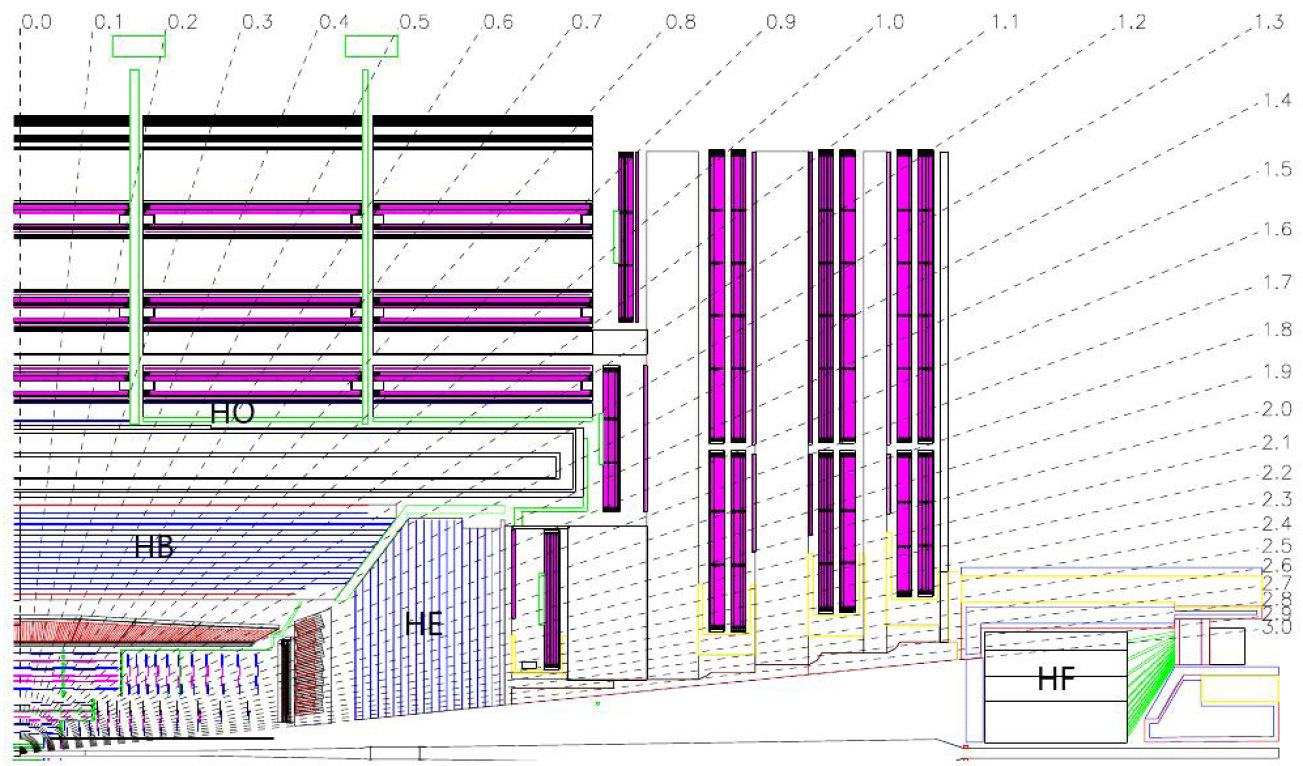
\includegraphics[width=0.9\textwidth]{figs/HCAL.png}
    \caption{CMS HCAL representation. \copyright CERN}
    \label{fig:hcal}
  \end{center}
\end{figure}

The HF design is very different from the rest of the HCAL subsystems. The most important challenge for the HF is the high resistance to radiation, while in the central rapidity region 100 GeV are deposited in average in the forward region is 760 GeV. For this reason it was chosen a Cherenkov detector made of quartz fibers with a steel absorber. The light produced in the HF is collected by photo multipliers. 

\subsection{Muon chambers}
\label{sec:muons}

The muon system of CMS is located at the most exterior layer of the detector  due to the penetration power of this particle. Muons are not stopped by the calorimeters and, with neutrinos, they are able to escape the detector. The muon chambers are placed in a cylinder around the HO and in disks on the end caps. Three main characteristics have been fulfilled from the design: efficient muon identification, precision measurement of muon charge and momentum and fast measurement to provide trigger capabilities. The moun chambers are made of three different subsystems:
\begin{itemize}
\item Drift Tubes Chambers (DT): Located in the region with $|\eta|<1.2$ and disposed in four layers. They consist of individual drift tubes of 50 $\mu$m of diameter anode wire with two electrode plates creating a drift electric field. The wall of the cell act as cathode. The cells are filled with a gas mixture, 85\% Argon and 15\% $\text{CO}_{2}$. The tubes are organized in plaques that are also organized in SuperLayers (SL) each one made of 4 plaques. The barrel is made of 250 DT's disposed in four cylinders separated by iron yokes. 
\item Cathode Strip Chambers (CSC): Installed in the end caps, provide a coverage up to $|\eta|=2.4$ from $|\eta|=0.9$. These chambers are multi-wire proportional chambers made of six planes of anode wires with 7 cathode planes. Four CSC stations are placed in each end cap. The wires are oriented in azimuthal direction while the cathode planes are radially oriented, allowing a complete measurement of the position of the particle. This system is able to measure with a precision between the 75 $\mu$m and 150$\mu$m.
\item Resistive Plate Chambers (RPC): This subsystem is made of gaseous parallel plate detectors. This detector is specially useful for triggering as it is very fast and have a good position resolution. There are 480 RPC distributed in 6 layers in the barrel with the DT and in 3 layers in the end caps with the CSC, and covers the region with $|\eta|<1.6$. 
\end{itemize}

On figure~\ref{fig:cmsmuon} can be found a representation of the muon system with the different components. The DT and CSC system cover $|\eta|<2.4$ without any gap. 

\begin{figure}[!Hhtbp]
  \begin{center}
    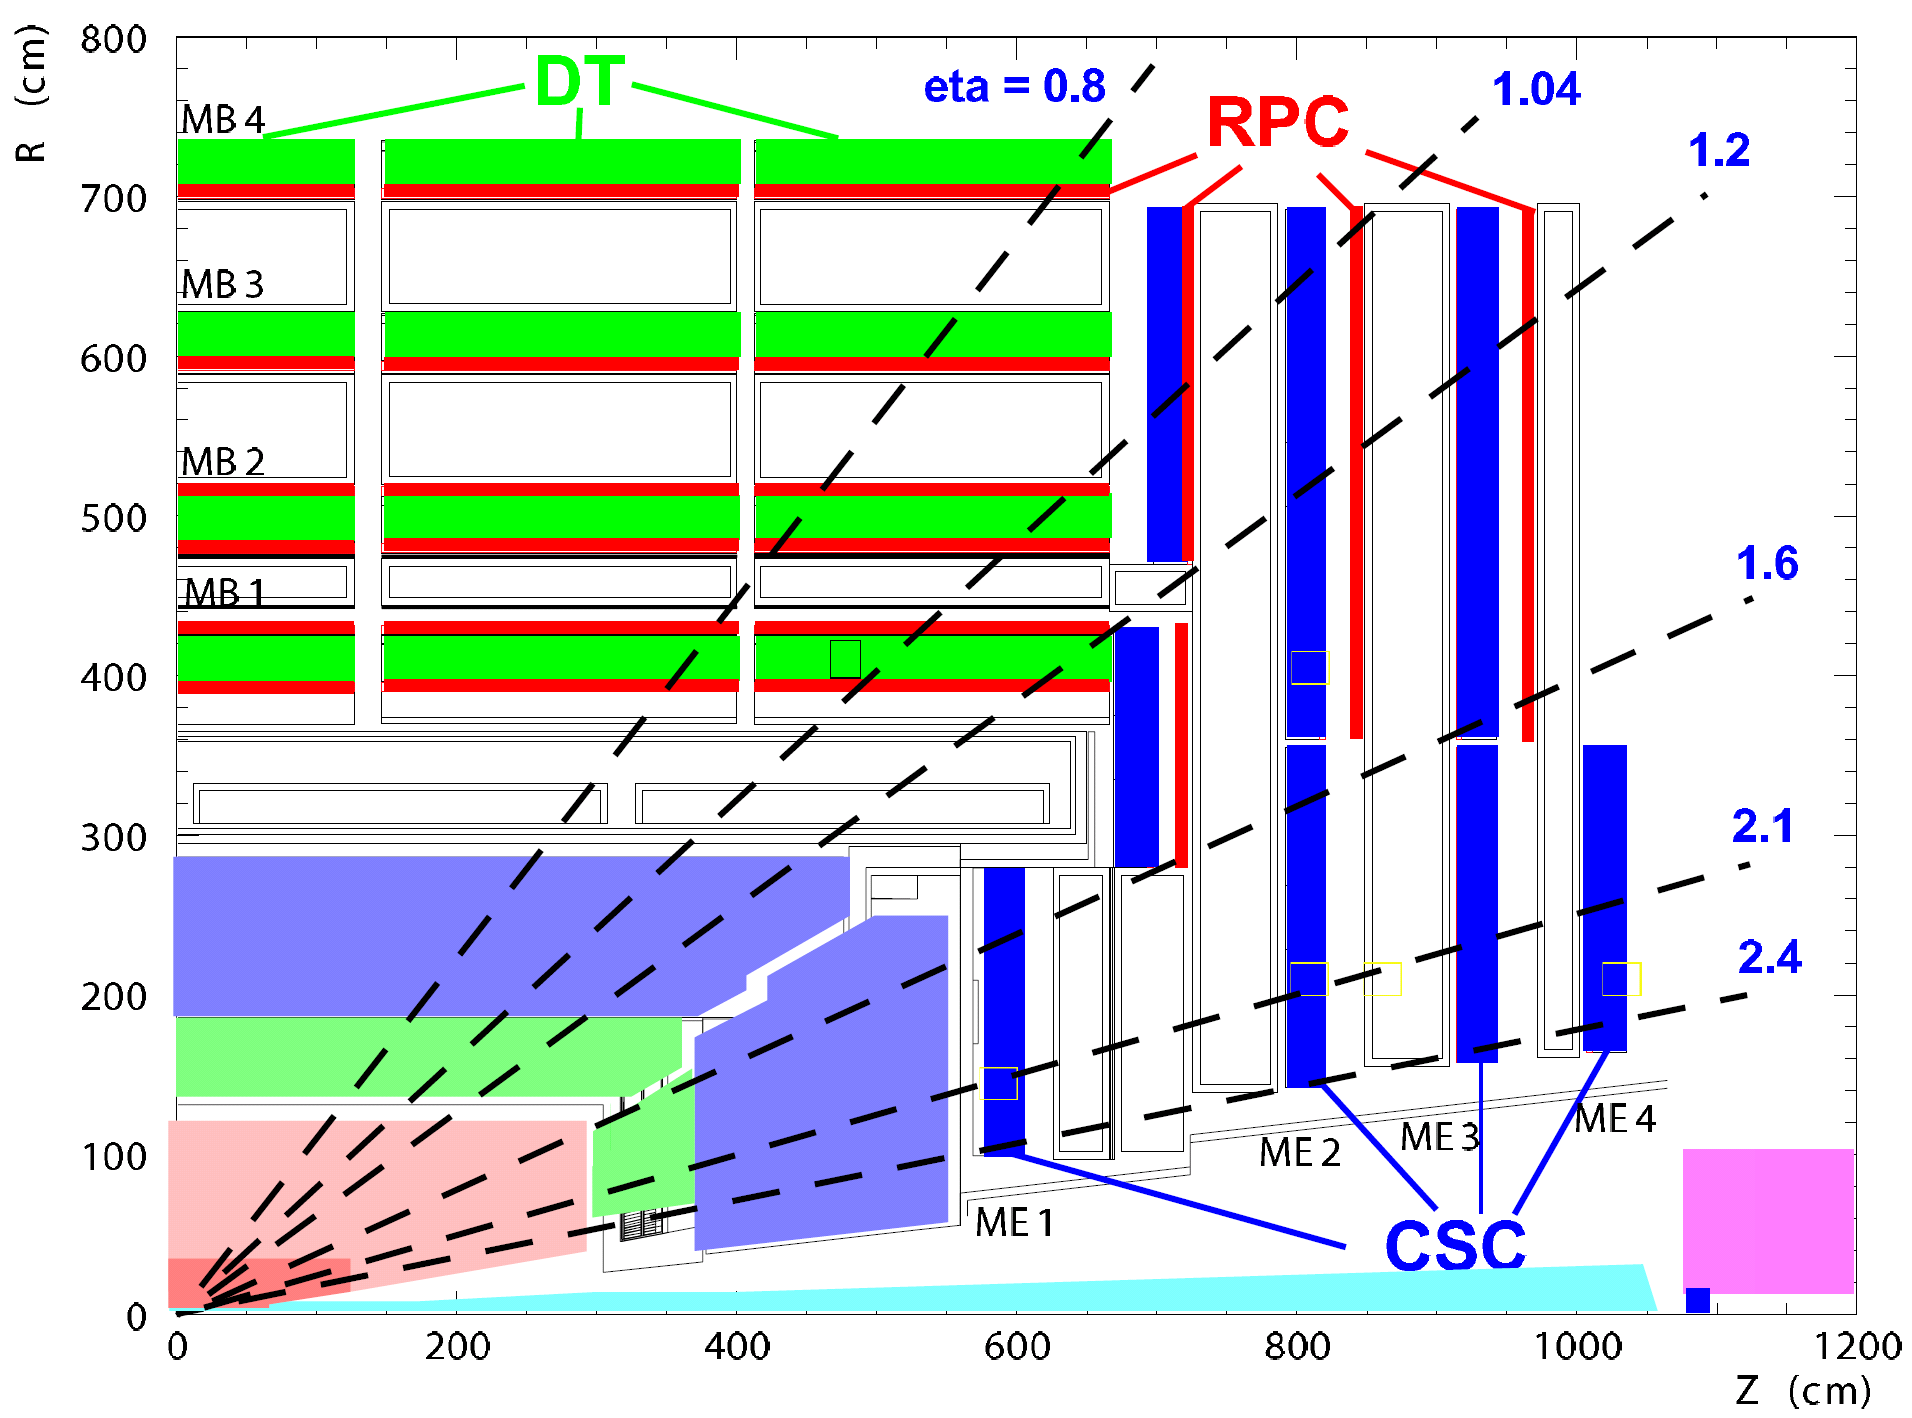
\includegraphics[width=0.9\textwidth]{figs/MuonDetector.png}
    \caption{CMS muon chambers representation. \copyright CERN}
    \label{fig:cmsmuon}
  \end{center}
\end{figure}

\subsection{Trigger}
\label{sec:trigger}

LHC has been designed to provide experiments with proton-proton collisions every 25 ns, meaning a frequency of 40 MHz. Each recorded event by CMS has a nominal size between 0.5 and 1 MB, what means a data flux of around $10^{9}\; \text{MB/s}= 1\text{PB/s}$ that is extremely big for transfer and for storing. Therefore, an on-line selection of events has to be done. The trigger system of CMS does this task in two fold, a level 1 (L1) and a high level trigger (HLT). The L1 is hardware based and the HLT is software based. 

From the searches conducted at CMS, the interesting events produced on proton-proton collisions for new physics searches are very rare. The enormous majority of events coming from proton-proton collisions correspond to well understood phenomena, while new physics events are 'exotic' with regards to the most common type of events. Then is interesting to keep only a part of the events, what actually easies the analysis afterward done over the data. 

The CMS trigger system is designed to keep only 100 kHz tops by the L1 and 300 Hz by the HLT. L1 is reducing the data flux by 2 orders of magnitude and the HLT another 3 orders of magnitude.

\subsubsection{Level 1 trigger}
\label{sec:L1}

The L1 is designed to trigger over coarse data coming from the calorimeters and muon chambers, holding data in pipe-lined memories in the front-end electronics. Therefore, relies on very fast reconstruction of objects coming from this subsystems: muons, electrons, photons, jets and missing energy. This reconstruction differs from the final reconstruction of the objects, for example a jet for the L1 consists on successive energy deposits in the ECAL and HCAL, while the off-line reconstruction take into account also the tracker information. 

The L1 starts from regional data coming from the subsystems which is afterward combined in order to build ranked trigger objects in localized regions of the detector. Global Muon and Calorimeter triggers sort the objects and send the best ranked to the Global Trigger (GT). Before the GT no events are rejected, is only with the GT that the selection is applied. The GT combines the information and can apply topological requirements and take a decision on keeping or disregarding the event. On figure~\ref{fig:l1} can be found the work-flow of the L1. 

\begin{figure}[!Hhtbp]
  \begin{center}
    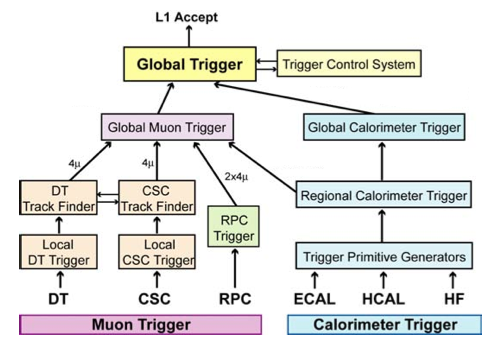
\includegraphics[width=0.9\textwidth]{figs/img_l1.png}
    \caption{L1 architecture. \copyright CERN}
    \label{fig:l1}
  \end{center}
\end{figure}

The L1 cards are distributed between the detector and an adjoin cavern at 90 m distance from the detector. The latency time L1 disposes between the collision and the taking of the decision is about 3.2 $\mu$s. Therefore, the front-end memory in the cards should be able to keep in memory up to 128 bunch crossings. 

\subsubsection{High Level Trigger}
\label{sec:HLT}

The HLT take as input the events accepted by the L1 and process them using farms of commercial processors. The HLT does additional operations on the selected events making it much slower than L1 processing. In particular, the HLT takes also into account the tracker information. Consequently, this system is able to take into consideration the whole information of the detector. However, the reconstruction of objects done by the HLT differs slightly from the final off-line reconstruction. The decision taking process takes around 40 ms, $10^{4}$ times more than for L1. 

The events selected by HLT are finally stocked on disks under several paths depending on the selection performed. There is a constant development of HLT paths focusing on different analysis requirements in order to obtain the best possible selection efficiency for specific signal types. 

%Add RUNII perspectives? Add section on dataset structure used by CMS?

%  LocalWords:  emittance ApparatuS
